\UseRawInputEncoding
\documentclass{article}

% Language setting
\usepackage[english]{babel}
\usepackage{pmboxdraw}

\usepackage[a4paper,top=2cm,bottom=2cm,left=3cm,right=3cm,marginparwidth=1.75cm]{geometry}

% Useful packages
\usepackage{amsmath}
\usepackage{tabularx}
\usepackage[T1]{fontenc}
\usepackage{graphicx}
\usepackage{listings}
\usepackage[colorlinks=true, allcolors=blue]{hyperref}

\title{Homework 04}

\author{Andrea Panceri 1884749}

\begin{document}
\maketitle

\section{Multi-Part computation}
We want a protocol that preserve privacy in this situation: we have n people ( with n > 1) that want to compare their salaries and find out what the average salary is. For guarantee the privacy we want that other people don't find our salary but only the average.
Now we start to describe the protocol for the general situation with n people and only after we demonstrate in practice the protocol with three people. For generate a shared key between pair of people,without have a third party, we will use diffie-hellman. In this way all the information exchanged by the pairs of people will be encrypted using the shared key, and therefore it will not be possible for other people to obtain sensitive information. We can use DH because in the requirements it has been said that there is not the man in the middle, otherwise this protocol is not secure. 
This will only be the first step to guarantee the confidentiality of the information exchanged between two people A and B, now let's start thinking about how to send the salary in a form that does not let others understand how much it is, but still manages to find the average. To do this each person will randomly divide their salary into n random numbers that add up to the sum, after doing this each number will be sent to a different person, so that everyone has a part of the salary of all n people. Subsequently, once a part of the salary has been obtained from all the n processes, the sum of all these values will be calculated and as a last step each process will send this calculated sum to all the other n processes.Finally, once all the sums have been obtained, a further sum of all these n values will be made and then divided by the number of people n, thus obtaining the average wages without ever having sent one's salary. As mentioned, the messages will be encrypted to guarantee confidentiality, but to avoid other types of attacks, such as replay attacks, the identity of the sender will be attached to each message, with a timestamp and a nounce. In this way we would have the security of the identity of the sender and the recipient every time. Fundamental is the fact that the messages are sent in the form of cipher text because otherwise by sniffing the messages of the LAN, the whole protocol would lose robustness, and also the fact of certifying the identity of the source is not negligible. After doing a very general and high-level discussion, let's show a case with n=3 to actually understand what the protocol does.\\
We have three people: Alice, Bob and Charlie with these salaries 100, 200 and 130. Using diffie hellman we will generate three session key \[K_{AB}, K_{BC}, K_{AC}\]After this we must generate three random number that that add up to the salary, for example:\\
Salary of A = 100 => 70 20 10\\
Salary of B = 200 => 150 50 0\\
Salary of C = 130 => 70 35 25\\
\begin{center}
\begin{tabular}{ |c|c|c|c| } 
\hline
 & A & B & C\\
\hline
A & 70 & 20 & 10\\
\hline
B & 150 & 50 & 0\\
\hline
C & 70 & 35 & 25\\
\hline
\end{tabular}
\end{center}
This is a tabular example of the messages exchanged, when each row is completed we can proceed to the next step of the protocol.\\
Now each person do the sum of the columns values A = 290, B = 105 and C = 35. Now each person send these values to the other people, obtain a new table:\\
\begin{center}
\begin{tabular}{ |c|c|c|c| } 
\hline
 & A & B & C\\
\hline
A & 290 & 290 & 290\\
\hline
B & 105 & 105 & 105\\
\hline
C & 35 & 35 & 35\\
\hline
\end{tabular}
\end{center}
Finally each person sum the values of his column and divide the result by the number of people, here by 3. The result for the three people is the same: 105 + 290 + 35 = 430 => 430/3 = 143,3 that is exactly the average of the salary, 100 + 200 + 130 = 430!\\
The protocol require a very high number of messages, but is really secure and guarantee the privacy, the most difficult part, aside the implementation of diffie hellman for generate the shared keys, is the generation of n random number that that add up to the salary, we can use for example this simple script in python:\\
\begin{lstlisting}
n = numberOfPeople
target = salary
while True:
    pick = random.sample(range(1, x), n)
    if sum(pick) == x:
        break
result = pick
\end{lstlisting}
after all these explanations the idea and the steps performed by the protocol should be clear, now we show graphically how it works for completeness:\\
\begin{center}
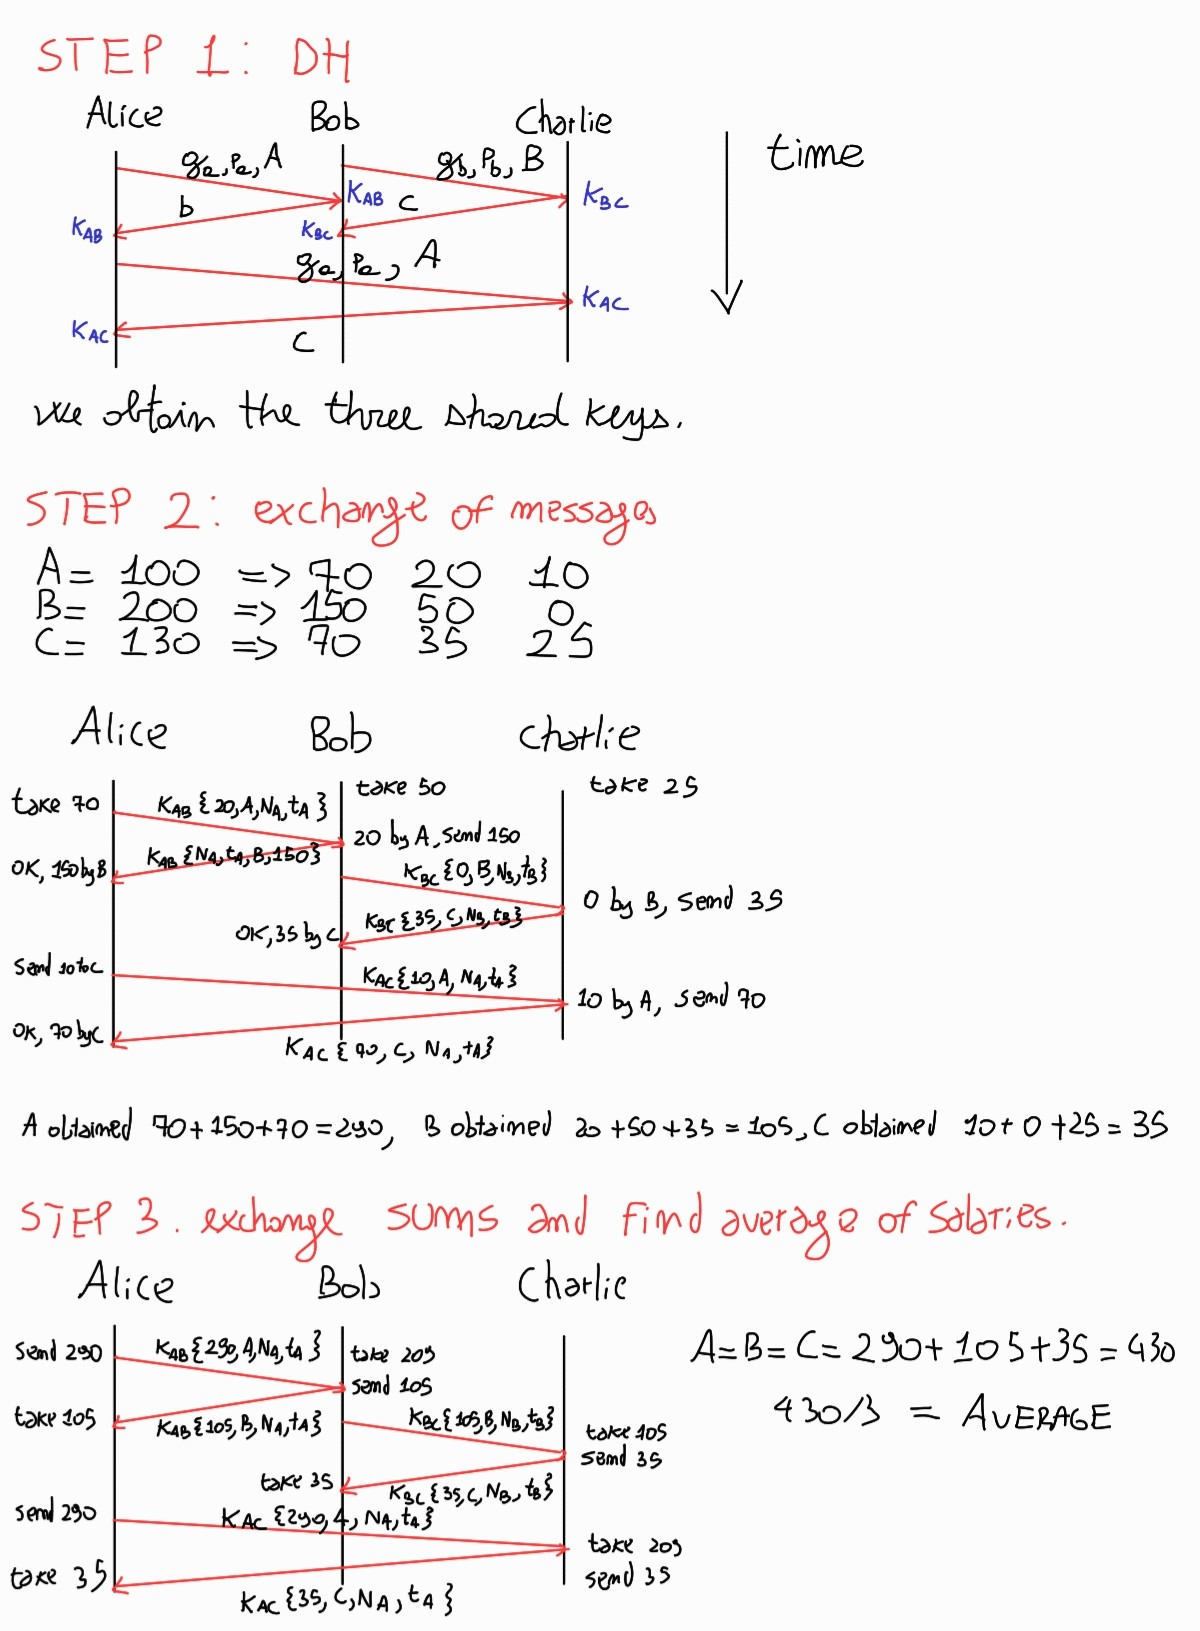
\includegraphics[scale=0.5]{HW04-1884749}
\end{center}
It is fundamental the concept that in Multi-Part computation the security isn't guarantee by the encryption, also by that, but the security is given by the union of the nounce, timestamp and identity of sender.
\end{document}
